% twocolumn を使うと2段組になる

%\documentclass[a4j,twocolumn]{jsarticle}        % -> platex
%\documentclass[a4j,twocolumn]{ujarticle}       % -> uplatex
\documentclass[uplatex]{jsarticle}   % -> uplatex + jsarticle

\usepackage{resume} % 他パッケージ,専用コマンド,余白の設定が書かれている

%%%%%%%%%%%%%%%%%%%%%%%%%%%%%%%%%%%%%%%%%%%%%%%%%%%%%%%%%%%%%%%%%%%%%%%%
% ヘッダ: イベント名,日付,所属,タイトル,氏名
%%%%%%%%%%%%%%%%%%%%%%%%%%%%%%%%%%%%%%%%%%%%%%%%%%%%%%%%%%%%%%%%%%%%%%%%

\pagestyle{plain}
\newcommand{\comment}[1]{}
\begin{document}
\twocolumn[
\beginheader{令和n年度 コンピュータサイエンス学部 輪講論文発表}{2022}{12}{22}{井上 研究室}
\title{弦楽合奏団の指揮体験にフィードバック機能を備えたVRコンテンツ}
\author{C0B20032 岡野 真士}
\endheader
]

\vspace{3mm}

 % 本番用ページ番号オフセット

%---------------------------------------------------------------------------
% 本文
%---------------------------------------------------------------------------


\section{はじめに}
 オーケストラを指揮する指揮者は、一生に一度はや ってみたい職業の一つと言われたこともある。

 指揮者の主な役割は、楽器を演奏する演奏者のま とめ役となること、また、演奏者の表現力を高めることにある。指揮に必要 な技術は、曲のテンポを決めること、音の強弱などを指 示すること、

 そこで、本研究では、指揮の基本である曲の拍子や テンポを体験者が思い通りに刻み、また、それができて いるかどうかを確認できるコンテンツを提案する。体験者が指揮に没 入して、様々なCG演出を活用できるよう VR 空間を利 用した。

\section{制作したコンテンツ}
 VR 空間上に制作した弦楽合奏団を図 1 に示す。楽 器アバタを使用して弦楽合奏団を表現した。

 \begin{figure}[H]
 \centering
 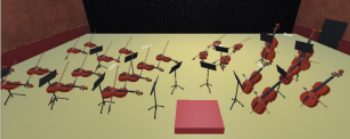
\includegraphics[clip,width=7cm]{gaikan.png}
 \caption{VR弦楽合奏団}\label{fig:hoge}
\end{figure}
 コンテンツの楽曲には、4 拍子の曲を用いた。指揮の体験者は両手に持ったコントローラを操作し、音量、曲の再生速度をそれぞれ 独立して制御するようにした。再生速度制御に必要なテンポは右手の指揮の動き から推定した。図 2 に 4 拍子の動きとそれを認識する仕 組みを示す。腕が I~IV の順に動いた場合に、4 拍子 が振れていると認識するようにした。テンポは、60 秒を 1 拍の動作にかかった時間で除算して推定した。

 4拍子を表現する腕の動きは、Y座標から検出した1拍の動作に着目し、1 拍の間にコントローラが左に移動した場合を1、右に移動した場合を2とし、それを順に記録していく。その並び方が、あらかじめ設定した 4 拍子の パターンに 1つでも該当すれば 4 拍子ができていると判 定した。

 \begin{figure}[H]
 \centering
 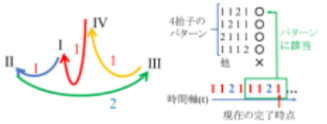
\includegraphics[clip,width=7cm]{hyousi.png}
 \caption{4拍子の動作判定の仕組み}\label{fig:hoge}
\end{figure}
 
 実験では、4拍子の成功や失敗にかかわらず、最後まで演奏を再生するようにした。 

 体験者が装着した HMD(Head Mounted Display)を 通して観察するコンテンツのシーンを図 3 に示す。

 \begin{figure}[H]
 \centering
 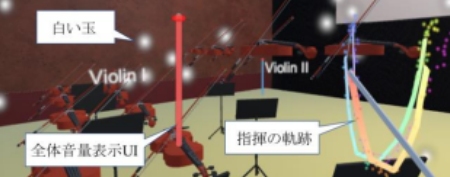
\includegraphics[clip,width=7cm]{sikumi.png}
 \caption{指揮を体験している様子}\label{fig:hoge}
\end{figure}

また、指揮の成功回数の積み重ねとして示す累積 回数に応じて、軌跡の色が「赤→黄→緑→青→紫→ 虹」と変化する。

\begin{figure}[H]
 \centering
 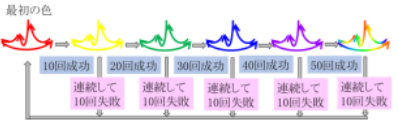
\includegraphics[clip,width=7cm]{sikisikumi.png}
 \caption{指揮軌跡の色の変化の規則}\label{fig:hoge}
\end{figure}

\section{予備実験}
\subsection{実験方法}
 本研究で提案した指揮動作と視覚演出の効果検証、 課題抽出を目的に大学生 12 名を被験者として予備実験を行った。
 実験では CG による視覚演出がないコンテンツを先 に体験し、その後、視覚演出のあるコンテンツを体験し てもらった。視覚演出なしの条件では、楽器アバタの動 きと、指揮の軌跡と色変化、白い玉の演出を止めた。一 方、体験者には指揮者のように感じてもらうため指揮棒 は表示し、また、実験で音量調整を必要としたため、全 体音量 UI とパート別音量 UI は表示するようにした。体 験後、アンケート調査を実施した。
\subsection{実験結果}
 視覚演出についての効果を調べた。視覚効果は、軌 跡表示と軌跡の色の変化、楽器のアニメーション、全体 音量の 4 つである。
 それぞれに対して、5 段階で回答してもらった。
\begin{figure}[H]
 \centering
 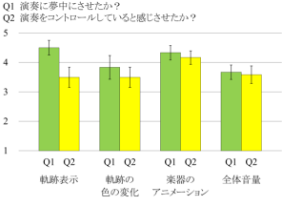
\includegraphics[clip,width=7cm]{yobi_1.png}
 \caption{資格演出に関するアンケート結果}
 \label{fig:hoge}
\end{figure}
結果から、「演奏をコントロールしていると感じさせたか」よりも「演奏に夢中にさせたか」の方が高い傾向を示し、この傾向は視覚演出に依存しない結果となった。

\section{コンテンツの改善}
前節の「課題抽出と解決策の検討」で述べた結果を もとに改善を施した。表 1 にコンテンツの改善点を示す。

\begin{table}[H]
 \centering
 \caption{コンテンツの改善点}\label{tab:fuga}
 \begin{tabular}{|c|l|}\hline
  改善項目 &  内容 \\
  \hline
  指標UI & お手本となる4拍子の図形を\\
  の表示& 体験者の司会正面に常時表示\\
  \hline
  軌跡の色 & 開始時の軌跡の色を赤から黄色へ変更。\\
  と軌跡の線形 & 4拍子失敗時に赤色で表示、かつ、軌跡\\ 
  状を変更&  の線の形状を実線から波線へ変更。\\
  \hline
  4拍子の& 失敗の判定を10回連続の条件から\\ 
  成功・失敗 & 7回連続の条件へ変更。失敗した後に \\
  の判定 & 成功の段階へ戻る回数を7回へ変更。\\
  \hline
  音の変調 & 4拍子に失敗時に\\
         & 再生されている曲を変調。\\
  \hline

  
 \end{tabular}
\end{table}

   4 拍子の指揮の動きや図形を確認できる指揮の 指標 UI を被験者の視界上に表示したときの様子を図6に示した。

\begin{figure}[H]
 \centering
 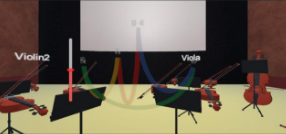
\includegraphics[clip,width=7cm]{sikiUI.png}
 \caption{4拍子の指揮指標UI}\label{fig:hoge}
\end{figure}

\section{実験}
\subsection{実験方法}
この実験では、コンテンツ体験中の被験者の集中力の推移を記録した。集中力の測定は、Neurosky社の脳波計である MindwaveMobile2 を用いて行った。


\subsection{実験結果}
4拍子の指揮をする際に指標 UI が効果的に作用し たかどうかについてアンケート調査を行った。図9に結 果を示す。被験者全員から役立ったとの回答が得られ、 指標 UI の表示は有効であることが分かった。 
\begin{figure}[H]
 \centering
 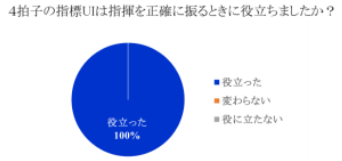
\includegraphics[clip,width=7cm]{UIkouka.png}
 \caption{指揮指標UIの効果}\label{fig:hoge}
\end{figure}

4拍子が正しく 振れているかどうかについて記録したデータを分析し定 量的に調べた。

\begin{figure}[H]
 \centering
 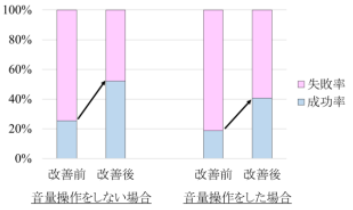
\includegraphics[clip,width=7cm]{sippairitu.png}
 \caption{コンテンツ改善前後の4拍子式の成功比率}\label{fig:hoge}
\end{figure}

\begin{figure}[H]
 \centering
 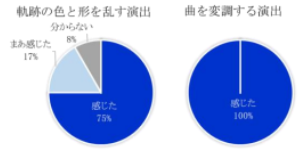
\includegraphics[clip,width=7cm]{miss.png}
 \caption{4拍子失敗時の四角的演出への城の結果}\label{fig:hoge}
\end{figure}

%---------------------------------------------------------------------------
% 本文終わり
%---------------------------------------------------------------------------

 % 参考文献
\bibliographystyle{junsrt}
\bibliography{ref}


\end{document}


%-----------------------------------------------------
% テンプレート
%------------------------------------------------------------------------------

%-----------
%% 箇条書き
%-----------
%\begin{itemize}
% \item
%\end{itemize}

%-------------------
%% 番号付き箇条書き
%-------------------
%\begin{enumerate}
% \item
%\end{enumerate}

%-----------
%% 図の表示
%-----------
%\begin{figure}[H]
% \centering
% \includegraphics[clip,width=7cm]{hoge.eps}
% \caption{図タイトル}\label{fig:hoge}
%\end{figure}

%-----------
%% 図の参照
%-----------
%\figref{fig:hoge}

%-----------
%% 表の作成
%-----------
%\begin{table}[H]
% \centering
% \caption{表タイトル}\label{tab:fuga}
% \begin{tabular}{|c|c|c|}\hline
%  hemo & piyo & fuga \\ \hline
%  hemo & piyo & fuga \\ \hline
% \end{tabular}
%\end{table}

%-----------
%% 表の参照
%-----------
%\tabref{tab:fuga}

%-----------
%% 参考文献
%-----------
%\begin{thebibliography}{9}
% \bibitem{piyo} 参考文献
%\end{thebibliography}

%-----------------
%% 参考文献の参照
%-----------------
%\cite{piyo}
